\let\negmedspace\undefined
\let\negthickspace\undefined
\documentclass[journal]{IEEEtran}
\usepackage[a5paper, margin=10mm, onecolumn]{geometry}
%\usepackage{lmodern} % Ensure lmodern is loaded for pdflatex
\usepackage{tfrupee} % Include tfrupee package

\setlength{\headheight}{1cm} % Set the height of the header box
\setlength{\headsep}{0mm}     % Set the distance between the header box and the top of the text

\usepackage{gvv-book}
\usepackage{gvv}
\usepackage{cite}
\usepackage{amsmath,amssymb,amsfonts,amsthm}
\usepackage{algorithmic}
\usepackage{graphicx}
\usepackage{textcomp}
\usepackage{xcolor}
\usepackage{txfonts}
\usepackage{listings}
\usepackage{enumitem}
\usepackage{mathtools}
\usepackage{gensymb}
\usepackage{comment}
\usepackage[breaklinks=true]{hyperref}
\usepackage{tkz-euclide}
\usepackage{listings}                                     
\def\inputGnumericTable{}                                 
\usepackage[utf8]{inputenc}                                
\usepackage{color}                                            
\usepackage{array}                                            
\usepackage{longtable}                                       
\usepackage{calc}                                             
\usepackage{multirow}                                         
\usepackage{hhline}                                           
\usepackage{ifthen}                                           
\usepackage{lscape}
\renewcommand{\thefigure}{\theenumi}
\renewcommand{\thetable}{\theenumi}
\setlength{\intextsep}{10pt} % Space between text and floats

\numberwithin{equation}{enumi}
\numberwithin{figure}{enumi}
\renewcommand{\thetable}{\theenumi}

% Marks the beginning of the document
\begin{document}
\bibliographystyle{IEEEtran}

\title{Question-9.6.13}
\author{EE24BTECH11048-NITHIN.K} 
%\maketitle
%\newpage
%\bigskip
{\let\newpage\relax\maketitle}
\textbf{Question:} \\
Find a particular solution for the differential equation $\frac{dy}{dx} + 2y\tan x = \sin x$ ; $y = 0$ when $x = \frac{\pi}{3}$ \\
\textbf{Solution:} \\
The original Differential Equation is \\
\begin{align}
	\frac{dy}{dx} + 2y\tan x = \sin x
\end{align}
\begin{align}
	\frac{dy}{dx} = \sin x - 2y\tan x
\end{align}
By Euler's approximation
\begin{align}                                                                   
	\frac{y_{n+1} - y_n}{dx} = \sin x_n - 2y_n\tan x_n 
\end{align}
Hence the difference equation is
\begin{align}
	y_{n+1} = y_n + dx\brak{\sin x_n - 2y_n\tan x_n}
\end{align}
Solution for the First Order Differential Equation:
\begin{align}
	\frac{dy}{dx} + 2y\tan x = \sin x
\end{align}
\begin{align}
	\frac{dy}{dx} + P\brak{x}y = Q\brak{x}
\end{align}
\begin{align}
	P\brak{x} = 2\tan x , Q\brak{x} = \sin x
\end{align}
\begin{align}
	IF = e^{\int2\tan x dx} = e^{2\ln|secx|} = \brak{\sec x}^2
\end{align}
By multiplying the Integrating Factor on both sides
\begin{align}
	\brak{\sec x}^2\frac{dy}{dx} + 2y\brak{\sec x}^2\tan(x) = \brak{\sec x}^2\sin x
\end{align}
\begin{align}
	\frac{d}{dx}\sbrak{\brak{\sec x}^2y} = \brak{\sec x}^2\sin x
\end{align}
and Integrating on both sides
\begin{align}
	\brak{\sec x}^2y = \int\brak{\sec x}^2\sin(x)dx
\end{align}
\begin{align}
	y = \cos x - 2{\cos x}^2
\end{align}

\begin{figure}[H]
    \centering
    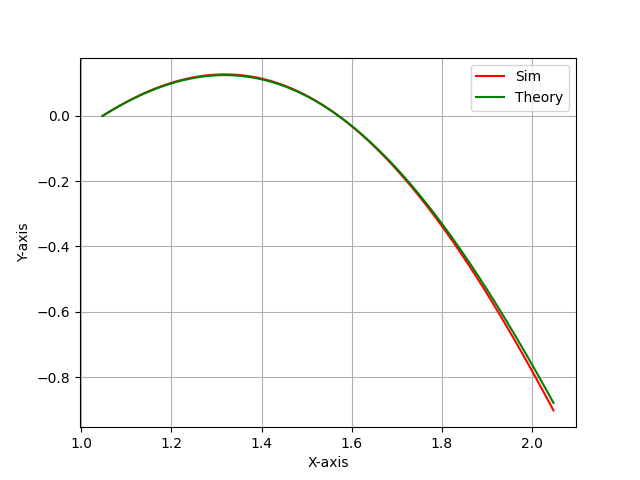
\includegraphics[width=0.8\textwidth]{figs/fig.png}
    \caption{Simulation VS Theoretical Plot.}
\end{figure}



\end{document}
